% Options for packages loaded elsewhere
% Options for packages loaded elsewhere
\PassOptionsToPackage{unicode}{hyperref}
\PassOptionsToPackage{hyphens}{url}
\PassOptionsToPackage{dvipsnames,svgnames,x11names}{xcolor}
%
\documentclass[
  letterpaper,
  DIV=11,
  numbers=noendperiod]{scrartcl}
\usepackage{xcolor}
\usepackage{amsmath,amssymb}
\setcounter{secnumdepth}{-\maxdimen} % remove section numbering
\usepackage{iftex}
\ifPDFTeX
  \usepackage[T1]{fontenc}
  \usepackage[utf8]{inputenc}
  \usepackage{textcomp} % provide euro and other symbols
\else % if luatex or xetex
  \usepackage{unicode-math} % this also loads fontspec
  \defaultfontfeatures{Scale=MatchLowercase}
  \defaultfontfeatures[\rmfamily]{Ligatures=TeX,Scale=1}
\fi
\usepackage{lmodern}
\ifPDFTeX\else
  % xetex/luatex font selection
\fi
% Use upquote if available, for straight quotes in verbatim environments
\IfFileExists{upquote.sty}{\usepackage{upquote}}{}
\IfFileExists{microtype.sty}{% use microtype if available
  \usepackage[]{microtype}
  \UseMicrotypeSet[protrusion]{basicmath} % disable protrusion for tt fonts
}{}
\makeatletter
\@ifundefined{KOMAClassName}{% if non-KOMA class
  \IfFileExists{parskip.sty}{%
    \usepackage{parskip}
  }{% else
    \setlength{\parindent}{0pt}
    \setlength{\parskip}{6pt plus 2pt minus 1pt}}
}{% if KOMA class
  \KOMAoptions{parskip=half}}
\makeatother
% Make \paragraph and \subparagraph free-standing
\makeatletter
\ifx\paragraph\undefined\else
  \let\oldparagraph\paragraph
  \renewcommand{\paragraph}{
    \@ifstar
      \xxxParagraphStar
      \xxxParagraphNoStar
  }
  \newcommand{\xxxParagraphStar}[1]{\oldparagraph*{#1}\mbox{}}
  \newcommand{\xxxParagraphNoStar}[1]{\oldparagraph{#1}\mbox{}}
\fi
\ifx\subparagraph\undefined\else
  \let\oldsubparagraph\subparagraph
  \renewcommand{\subparagraph}{
    \@ifstar
      \xxxSubParagraphStar
      \xxxSubParagraphNoStar
  }
  \newcommand{\xxxSubParagraphStar}[1]{\oldsubparagraph*{#1}\mbox{}}
  \newcommand{\xxxSubParagraphNoStar}[1]{\oldsubparagraph{#1}\mbox{}}
\fi
\makeatother


\usepackage{longtable,booktabs,array}
\usepackage{calc} % for calculating minipage widths
% Correct order of tables after \paragraph or \subparagraph
\usepackage{etoolbox}
\makeatletter
\patchcmd\longtable{\par}{\if@noskipsec\mbox{}\fi\par}{}{}
\makeatother
% Allow footnotes in longtable head/foot
\IfFileExists{footnotehyper.sty}{\usepackage{footnotehyper}}{\usepackage{footnote}}
\makesavenoteenv{longtable}
\usepackage{graphicx}
\makeatletter
\newsavebox\pandoc@box
\newcommand*\pandocbounded[1]{% scales image to fit in text height/width
  \sbox\pandoc@box{#1}%
  \Gscale@div\@tempa{\textheight}{\dimexpr\ht\pandoc@box+\dp\pandoc@box\relax}%
  \Gscale@div\@tempb{\linewidth}{\wd\pandoc@box}%
  \ifdim\@tempb\p@<\@tempa\p@\let\@tempa\@tempb\fi% select the smaller of both
  \ifdim\@tempa\p@<\p@\scalebox{\@tempa}{\usebox\pandoc@box}%
  \else\usebox{\pandoc@box}%
  \fi%
}
% Set default figure placement to htbp
\def\fps@figure{htbp}
\makeatother





\setlength{\emergencystretch}{3em} % prevent overfull lines

\providecommand{\tightlist}{%
  \setlength{\itemsep}{0pt}\setlength{\parskip}{0pt}}



 


\KOMAoption{captions}{tableheading}
\makeatletter
\@ifpackageloaded{caption}{}{\usepackage{caption}}
\AtBeginDocument{%
\ifdefined\contentsname
  \renewcommand*\contentsname{Table of contents}
\else
  \newcommand\contentsname{Table of contents}
\fi
\ifdefined\listfigurename
  \renewcommand*\listfigurename{List of Figures}
\else
  \newcommand\listfigurename{List of Figures}
\fi
\ifdefined\listtablename
  \renewcommand*\listtablename{List of Tables}
\else
  \newcommand\listtablename{List of Tables}
\fi
\ifdefined\figurename
  \renewcommand*\figurename{Figure}
\else
  \newcommand\figurename{Figure}
\fi
\ifdefined\tablename
  \renewcommand*\tablename{Table}
\else
  \newcommand\tablename{Table}
\fi
}
\@ifpackageloaded{float}{}{\usepackage{float}}
\floatstyle{ruled}
\@ifundefined{c@chapter}{\newfloat{codelisting}{h}{lop}}{\newfloat{codelisting}{h}{lop}[chapter]}
\floatname{codelisting}{Listing}
\newcommand*\listoflistings{\listof{codelisting}{List of Listings}}
\makeatother
\makeatletter
\makeatother
\makeatletter
\@ifpackageloaded{caption}{}{\usepackage{caption}}
\@ifpackageloaded{subcaption}{}{\usepackage{subcaption}}
\makeatother
\usepackage{bookmark}
\IfFileExists{xurl.sty}{\usepackage{xurl}}{} % add URL line breaks if available
\urlstyle{same}
\hypersetup{
  pdftitle={Simulation Challenge},
  colorlinks=true,
  linkcolor={blue},
  filecolor={Maroon},
  citecolor={Blue},
  urlcolor={Blue},
  pdfcreator={LaTeX via pandoc}}


\title{Simulation Challenge}
\usepackage{etoolbox}
\makeatletter
\providecommand{\subtitle}[1]{% add subtitle to \maketitle
  \apptocmd{\@title}{\par {\large #1 \par}}{}{}
}
\makeatother
\subtitle{Generative Models and Monte Carlo Simulation}
\author{}
\date{}
\begin{document}
\maketitle


\begin{enumerate}
\def\labelenumi{\arabic{enumi}.}
\tightlist
\item
  \textbf{Expected Value Analysis:} What is the ``expected value'' of
  your account balance after 1 coin flip for the original game?
\end{enumerate}

\subsection{The expected value of the account balance after 1 coin flip
for the original game is \$1000 * (0.5 * 1.5 + 0.5 * 0.6) = \$1050.
Therefore, the expected value is positive and
\$1050.}\label{the-expected-value-of-the-account-balance-after-1-coin-flip-for-the-original-game-is-1000-0.5-1.5-0.5-0.6-1050.-therefore-the-expected-value-is-positive-and-1050.}

\phantomsection\label{q1-expected-value}
\begin{verbatim}
Starting balance: $1,000
Expected value after one flip: $1,050
\end{verbatim}

\begin{enumerate}
\def\labelenumi{\arabic{enumi}.}
\setcounter{enumi}{1}
\tightlist
\item
  \textbf{Expectation vs.~Reality:} Is the expected value positive or
  negative? Do you expect your account to be worth more or less than
  \$1,000 based on this result?
\end{enumerate}

\subsection{The expected value is positive with a gain of \$50.
Therefore, I expect my account to be worth more than
\$1,000.}\label{the-expected-value-is-positive-with-a-gain-of-50.-therefore-i-expect-my-account-to-be-worth-more-than-1000.}

\phantomsection\label{q2-expectation-vs-reality}
\begin{verbatim}
Expected value: $1,050
Is expected value positive? Yes
Expected balance > $1,000? Yes
\end{verbatim}

\begin{enumerate}
\def\labelenumi{\arabic{enumi}.}
\setcounter{enumi}{2}
\tightlist
\item
  \textbf{Single Simulation:} Run one simulation showing the dynamics of
  your account balance over time. Make an object-oriented matplotlib OR
  ggplot2 plot showing your simulated account balance over time (i.e.~as
  you age). Comment on the results, are you happy?
\end{enumerate}

\subsection{Answer: Below is a single simulation of the original game
(multiplicative: +50\% on heads, -40\% on tails) over 30 years with an
object-oriented Matplotlib plot. The final balance can vary greatly; a
single path can end very high or very low, so happiness depends on the
particular sequence of flips. Overall, years 10 to mid 20, I am not too
happy because my account balance is very low. Moreover, starting with
\$!,000 at age 0 and ending with \$200 at age 30, I lost over \$800
which is not a good outcome of the simulation; I would have preferred to
see my account balance grow over
time.}\label{answer-below-is-a-single-simulation-of-the-original-game-multiplicative-50-on-heads--40-on-tails-over-30-years-with-an-object-oriented-matplotlib-plot.-the-final-balance-can-vary-greatly-a-single-path-can-end-very-high-or-very-low-so-happiness-depends-on-the-particular-sequence-of-flips.-overall-years-10-to-mid-20-i-am-not-too-happy-because-my-account-balance-is-very-low.-moreover-starting-with-000-at-age-0-and-ending-with-200-at-age-30-i-lost-over-800-which-is-not-a-good-outcome-of-the-simulation-i-would-have-preferred-to-see-my-account-balance-grow-over-time.}

\pandocbounded{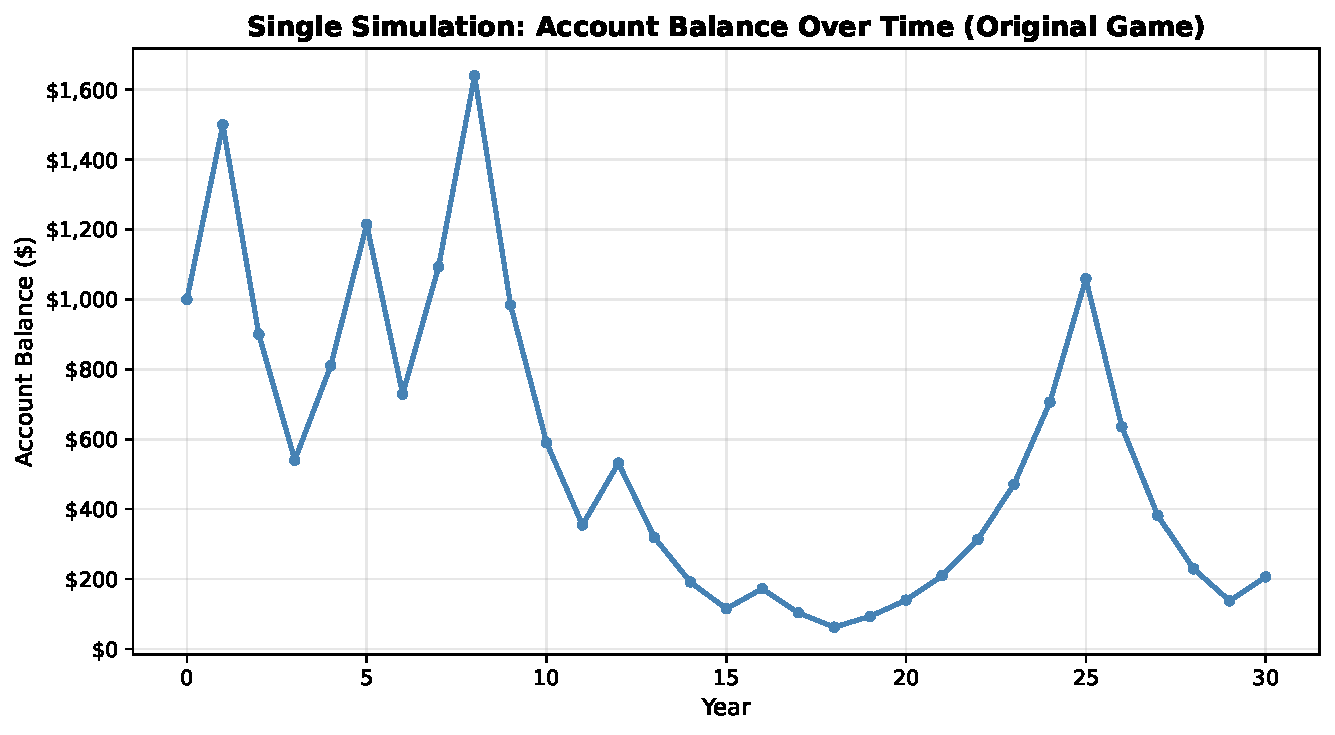
\includegraphics[keepaspectratio]{index_files/figure-pdf/q3-single-simulation-output-1.pdf}}

\begin{verbatim}
Final balance after 30 years: $205.89
\end{verbatim}

\subsubsection{Questions to Answer for 85\% Grade on
Challenge}\label{questions-to-answer-for-85-grade-on-challenge}

\begin{enumerate}
\def\labelenumi{\arabic{enumi}.}
\setcounter{enumi}{3}
\tightlist
\item
  \textbf{Multiple Simulations:} Run 100 simulations modelling the
  dynamics of your account balance over time. Make an object-oriented
  matplotlib OR ggplot2 plot showing a probability distribution of the
  100 simulatedaccount balance at age 55. Comment on the results, are
  you happy? Why or why not?
\end{enumerate}

\subsection{Answer: Below are 100 simulations of the original game over
30 years (age 25 to 55) with a Matplotlib histogram showing the
distribution of final balances. I did buckets for every \$500 and for
any value above \$10,000, I placed it in that bucket. I am not very
happy with the results because there is a 70\% chance that my account
balance by age 55 will be below the \$1,000 threshold. Therefore, I am
not a risky player so there is no point of me trying to play this game
since most likely, I will end up losing money. There is a small chance
to hit the lottery and end up with over \$10,000, but that risk is not
worth it
statistically.}\label{answer-below-are-100-simulations-of-the-original-game-over-30-years-age-25-to-55-with-a-matplotlib-histogram-showing-the-distribution-of-final-balances.-i-did-buckets-for-every-500-and-for-any-value-above-10000-i-placed-it-in-that-bucket.-i-am-not-very-happy-with-the-results-because-there-is-a-70-chance-that-my-account-balance-by-age-55-will-be-below-the-1000-threshold.-therefore-i-am-not-a-risky-player-so-there-is-no-point-of-me-trying-to-play-this-game-since-most-likely-i-will-end-up-losing-money.-there-is-a-small-chance-to-hit-the-lottery-and-end-up-with-over-10000-but-that-risk-is-not-worth-it-statistically.}

\pandocbounded{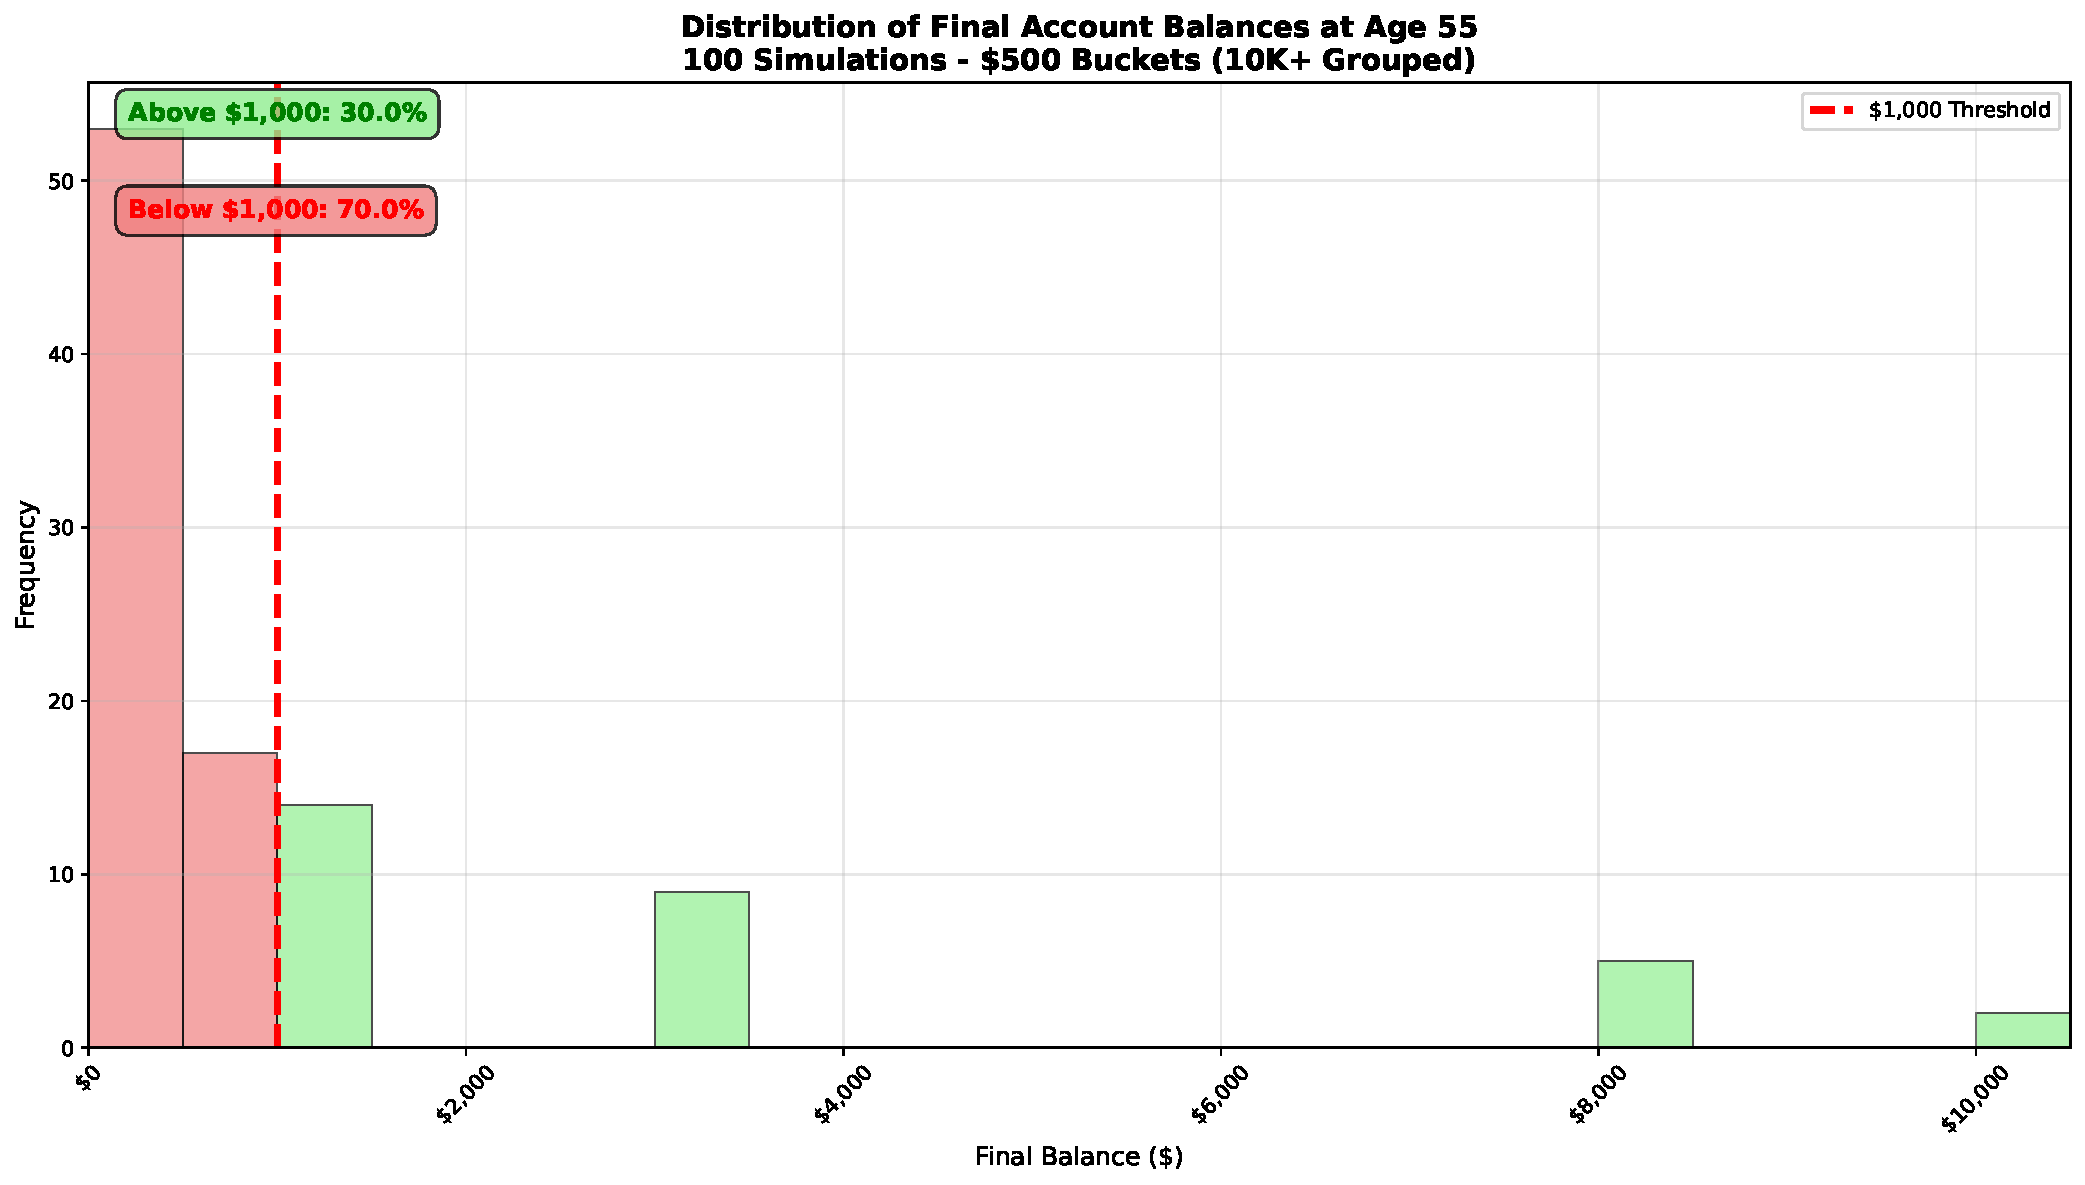
\includegraphics[keepaspectratio]{index_files/figure-pdf/q4-multiple-simulations-output-1.pdf}}

\begin{verbatim}
Summary Statistics (100 simulations):
Mean final balance: $1,718.87
Median final balance: $205.89
Probability above $1,000: 0.300
Maximum balance: $50,266.39
Minimum balance: $0.13
\end{verbatim}

\subsubsection{Questions to Answer for 95\% Grade on
Challenge}\label{questions-to-answer-for-95-grade-on-challenge}

\begin{enumerate}
\def\labelenumi{\arabic{enumi}.}
\setcounter{enumi}{4}
\tightlist
\item
  \textbf{Probability Analysis:} Based on the 100 simulations above,
  what is the probability that your account balance will be greater than
  \$1,000 at age 55?
\end{enumerate}

\subsection{Answer: Based on the 100 simulations from Question 4, the
probability of ending above \$1,000 at age 55 is 30\%. This means that
the probability you end up with less than \$1,000 will be 70\% which is
not a great outcome for the
player.}\label{answer-based-on-the-100-simulations-from-question-4-the-probability-of-ending-above-1000-at-age-55-is-30.-this-means-that-the-probability-you-end-up-with-less-than-1000-will-be-70-which-is-not-a-great-outcome-for-the-player.}

\phantomsection\label{q5-probability-analysis}
\begin{verbatim}
Results from 100 simulations:
Simulations ending above $1,000: 30
Simulations ending below $1,000: 70

Probability of ending above $1,000: 0.300 (30.0%)
Probability of ending below $1,000: 0.700 (70.0%)

Answer: The probability that your account balance will be greater than $1,000 at age 55 is 30.0%
\end{verbatim}

\subsubsection{Questions to Answer for 100\% Grade on
Challenge}\label{questions-to-answer-for-100-grade-on-challenge}

\begin{enumerate}
\def\labelenumi{\arabic{enumi}.}
\setcounter{enumi}{5}
\tightlist
\item
  \textbf{Strategy Comparison:} Run 100 simulations for the modified
  game strategy shown below in
  \textbf{?@exm-ErgodicityEconomicsExampleModified}. What is the
  probability that your account balance will be greater than \$10,000 at
  age 55? Is this probability higher or lower than the probability in
  the original game?
\end{enumerate}

\subsection{Answer: Below are 100 simulations of the modified game
strategy (betting 50\% of balance each round) compared to the original
game. The modified strategy shows different dynamics due to the fixed
betting percentage. What I can see from the graph is that the
probability that my account balance is greater than \$10,000 is lower in
the modified game than the original game. There is a 3\% chance that I
will end up with over \$10,000 in original game compared to a 1\% chance
I will end up with over \$10,000 in the modified game. However, if the
threshold is \$1,000, the probability is much higher in the modified
game as we can see in the graph there is higher amount of clusters above
\$1,000 compared to the original
game.}\label{answer-below-are-100-simulations-of-the-modified-game-strategy-betting-50-of-balance-each-round-compared-to-the-original-game.-the-modified-strategy-shows-different-dynamics-due-to-the-fixed-betting-percentage.-what-i-can-see-from-the-graph-is-that-the-probability-that-my-account-balance-is-greater-than-10000-is-lower-in-the-modified-game-than-the-original-game.-there-is-a-3-chance-that-i-will-end-up-with-over-10000-in-original-game-compared-to-a-1-chance-i-will-end-up-with-over-10000-in-the-modified-game.-however-if-the-threshold-is-1000-the-probability-is-much-higher-in-the-modified-game-as-we-can-see-in-the-graph-there-is-higher-amount-of-clusters-above-1000-compared-to-the-original-game.}

\pandocbounded{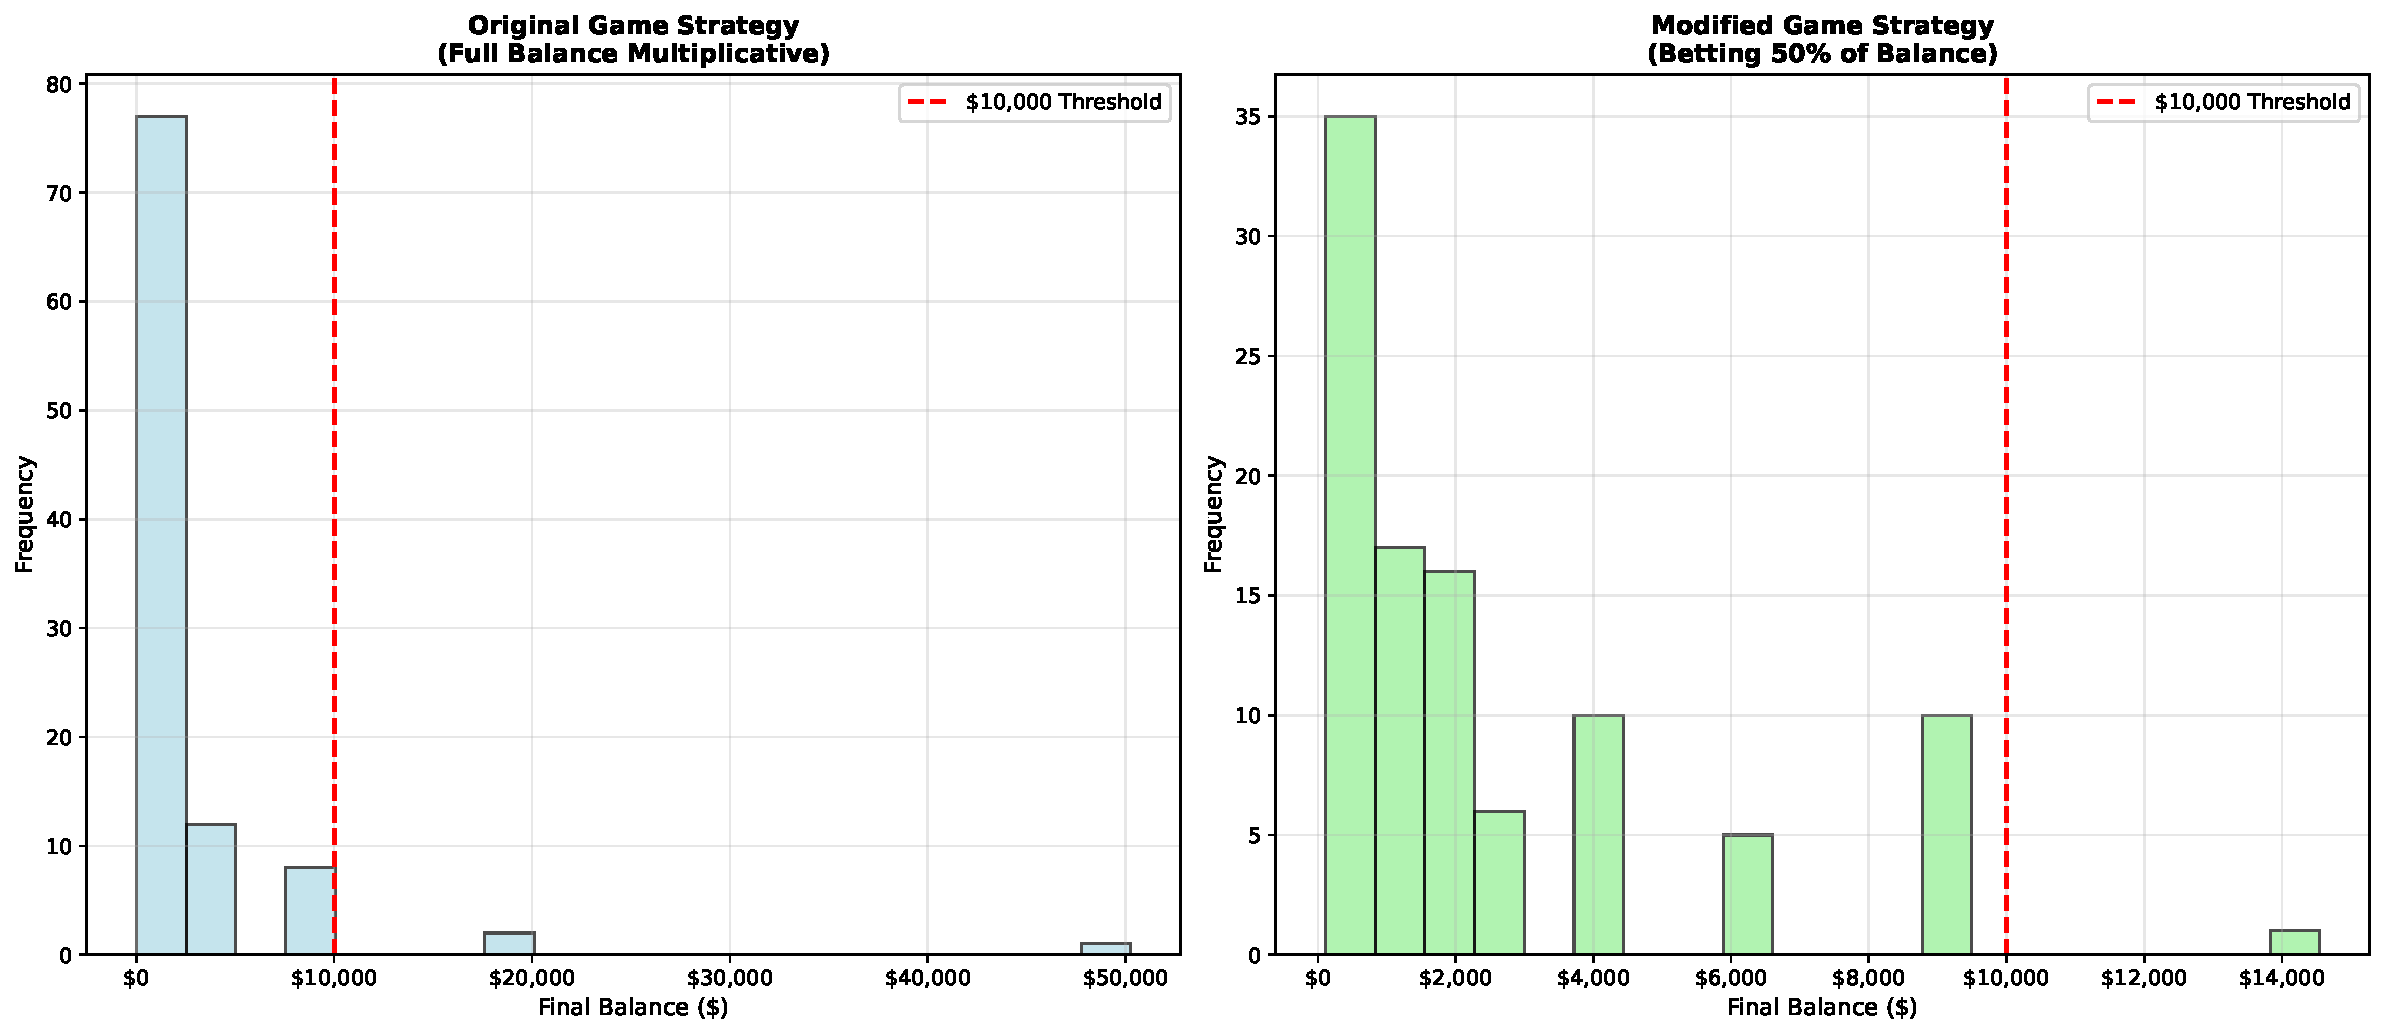
\includegraphics[keepaspectratio]{index_files/figure-pdf/q6-strategy-comparison-output-1.pdf}}

\begin{verbatim}
Strategy Comparison Results:
Original Game - Probability above $10,000: 0.030 (3.0%)
Modified Game - Probability above $10,000: 0.010 (1.0%)

Answer: The probability of ending above $10,000 is 1.0% for the modified game.
This is LOWER than the original game (3.0%).
\end{verbatim}




\end{document}
